\title{Chapter 4, Section 2. Exercises 1, 2, and 4 through 9}
\author{
	MTH 594, Prof. Mikael Vejdemo-Johansson \\
	Differential Geometry Independent Study \\
	\\
	Matthew Connelly \\
}
\date{\today}



\documentclass[12pt]{article}

\usepackage[top=.5in, bottom=.75in, left=1in, right=1in]{geometry}
\usepackage{amssymb}
\usepackage{amsmath}
\usepackage{graphicx}
\usepackage{subcaption}


\begin{document}
\maketitle

\section*{Exercise 4.2.2}
Verify that the the six surface patches for $S^2$ in Exercise 4.1.2 are regular. Calculate the transition maps between them and verify that these maps are smooth.

\vspace{1cm}
\hrule
\vspace{1cm}
\noindent
\underline{Preliminary definitions and clarification:}\\\\
This problem is referring to surface $S^2$, which is a sphere that has been split into six \\ surface patches that look like domes. Only two of these patches would be needed to complete the \emph{image} of the surface (but not the surface in its entirety). The parametrization $\sigma$ maps $u,v \in U$ to $S^2 \cap W$ by the following definition:
$$
\sigma^{x}_{\pm}(u,v) = (\pm \sqrt{1-u^2-v^2}, u ,v)
$$
\indent
A near-identical definition is used for the $\pm y$ and $\pm z$ patches.\\
\indent
All six patches can be visualized as the following four domes (or even the just the first two) through the appropriate rotation/orientation:
\begin{figure}[h!]
  \centering
      \begin{subfigure}[b]{0.5\linewidth}
    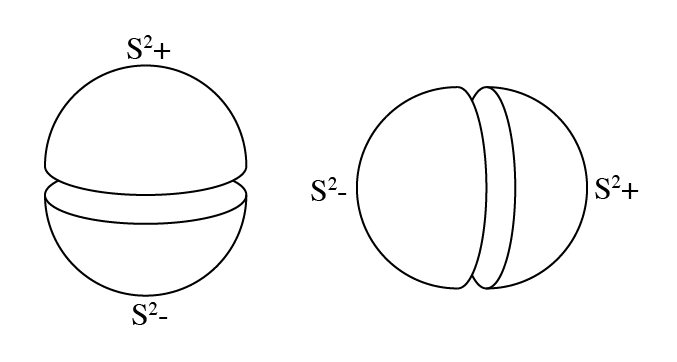
\includegraphics[width=\linewidth]{./assets/4-2-2/s2-patches.png}
  \end{subfigure}
  \end{figure}
  \\
These six patches (four of which could be depicted as above) are essentially nested, creating an overlap between all six and covering the open bounds of each other (covering the edge made by the "slice"), making an atlas for the entirety of $S^2$.

\clearpage

\underline{Verifying regularity of $\sigma$:}\\\\



\end{document}
This is never printed
